\documentclass[tikz,border=10pt]{standalone}
\begin{document}
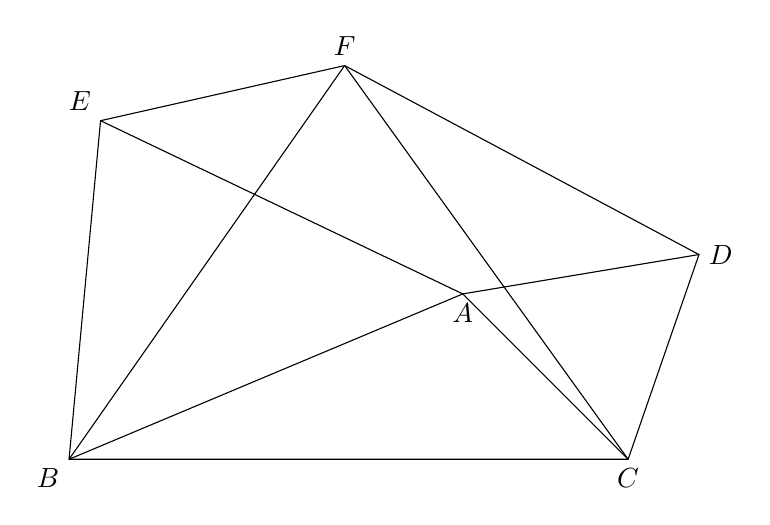
\begin{tikzpicture}[line cap=round,line join=round]

\coordinate (B) at (0,0);
\coordinate (E) at (0.4,4.3);
\coordinate (F) at (3.5,5.0);
\coordinate (A) at (5.0,2.1);
\coordinate (C) at (7.1,0.0);
\coordinate (D) at (8.0,2.6);

\draw (E) -- (F) -- (D) -- (C) -- (B) -- (E);
\draw (B) -- (F);
\draw (F) -- (C);
\draw (E) -- (A) -- (C);
\draw (B) -- (A) -- (D);

\node[above left] at (E) {$E$};
\node[above] at (F) {$F$};
\node[below left] at (B) {$B$};
\node[below] at (C) {$C$};
\node[right] at (D) {$D$};
\node[below] at (A) {$A$};

\end{tikzpicture}
\end{document}
